%% Slides for ".NET Programming" by Chunyu Wang <chunyu@hit.edu.cn> %% -*- coding: utf-8 -*-

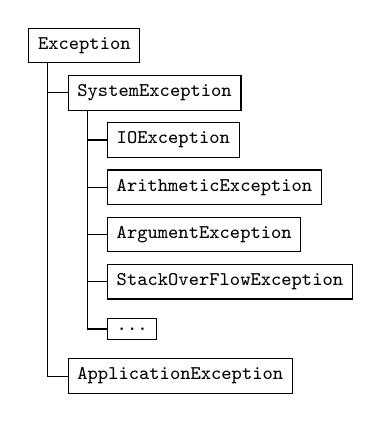
\begin{tikzpicture}
  \tikzstyle{every node}=[anchor=west, draw,fill=white, font=\ttfamily\scriptsize]
  \node at (0,5) (a) {Exception};
  \node at (.5,4.4) (b) {SystemException};
  \node at (1,3.8) (b1) {IOException};
  \node at (1,3.2) (b2) {ArithmeticException};
  \node at (1,2.6) (b3) {ArgumentException};
  \node at (1,2)   (b4) {StackOverFlowException};
  \node at (1,1.4) (b5) {\mbox{}...};
  \node at (.5,.8) (c) {ApplicationException};

  \draw (a.south west) +(right:.25cm) |- (b);
  \draw (a.south west) +(right:.25cm) |- (c);

  \foreach \a in {b1,b2,b3,b4,b5}
  \draw (b.south west) +(right:.25cm) |- (\a);
\end{tikzpicture}
